%Version 3.1 December 2024
% SNAM Journal Submission -- REVISED MANUSCRIPT
% Contextual Hashtag Weighting for Social Media Clustering
%%%%%%%%%%%%%%%%%%%%%%%%%%%%%%%%%%%%%%%%%%%%%%%%%%%%%%%%%%%%%%%%%%%%%%

\documentclass[pdflatex,sn-mathphys-num]{sn-jnl}% Math and Physical Sciences Numbered Reference Style

%%%% Standard Packages
\usepackage{graphicx}%
\usepackage{multirow}%
\usepackage{amsmath,amssymb,amsfonts}%
\usepackage{amsthm}%
\usepackage{textcomp}%
\usepackage{booktabs}%
\usepackage{url}%
\usepackage{xcolor}%

\raggedbottom

\begin{document}

\title[Contextual Hashtag Weighting for Social Media Clustering]{Contextual Hashtag Weighting for Social Media Clustering: A Zero-Energy Framework Evaluated Across Two Domains}

%%=============================================================%%
%% Author Information
%%=============================================================%%

\author*[1]{\fnm{Krishnan} \sur{Batri}}\email{krishnan.batri@gmail.com}

\author[2]{\fnm{Rajermani} \sur{Thinakaran}}\email{rajermani.thina@newinti.edu.my}

\author[3]{\fnm{Celal} \sur{Alagöz}}\email{alagozc@sivas.edu.tr}

\author[4]{\fnm{P.} \sur{Sasikumar}}\email{sasikumar.p@buv.edu.vn}

\author[4]{\fnm{M. Viju} \sur{Prakash}}\email{viju.m@buv.edu.vn}

\author[1]{\fnm{S.} \sur{Lakshmi}}\email{lakshmibatri@gmail.com}

\author[3]{\fnm{Sivaram} \sur{Murugan}}\email{sivaram.murugan@sivas.edu.tr}

%%=============================================================%%
%% Affiliations
%%=============================================================%%

\affil*[1]{\orgdiv{Department of Computer Science and Engineering}, \orgname{Sharda University}, \orgaddress{\city{Greater Noida}, \postcode{201310}, \state{Uttar Pradesh}, \country{India}}}

\affil[2]{\orgdiv{Faculty of Data Science and Information Technology}, \orgname{INTI International University}, \orgaddress{\state{Negeri Sembilan}, \country{Malaysia}}}

\affil[3]{\orgdiv{Department of Computer Engineering}, \orgname{Sivas University of Science and Technology}, \orgaddress{\city{Sivas}, \postcode{58000}, \country{Türkiye}}}

\affil[4]{\orgdiv{School of Computing and Innovative Technologies}, \orgname{British University Vietnam}, \orgaddress{\city{Ecopark}, \state{Hung Yen}, \country{Vietnam}}}

%%=============================================================%%
%% Abstract
%%=============================================================%%

\abstract{Social media clustering methods usually treat hashtags as independent features with intrinsic, frequency-based importance, overlooking the contextual relationships that shape their meaning and use. This paper proposes a Zero-Energy Baseline framework in which hashtag importance is derived entirely from contextual interactions rather than frequency-based priors. The framework decomposes contextual influence into three energy components: hashtag--hashtag interactions via co-occurrence and semantic similarity, text--hashtag coupling through embedding alignment, and engagement-scaled temporal activity. A Lifecycle Equivalence rule assigns zero temporal energy to hashtags that are new or have been dormant beyond a threshold, so that both are treated identically.

We evaluate the framework on the held-out test splits of two Twitter datasets: COVID-19 health discourse (6,293 test tweets, 897 hashtags, April 2020--June 2021) and US Election 2020 political discourse (182,549 test tweets, 16,841 hashtags, October--November 2020). The same relative pattern appears in both datasets. Within the tested range $K \in \{2,5,10,15,20\}$, Silhouette is highest at $K=20$ for COVID-19 (a 45\% gain over $K=2$), whereas for Election 2020 the values at $K=2$ and $K=20$ lie within run-to-run variation; the Davies--Bouldin index favours $K=15$ and $K=10$ respectively. Contextual hashtag features obtain higher Silhouette than TF-IDF text features ($\Delta S = 0.26$ and $0.12$), concatenated hashtag--TF-IDF features ($\Delta S = 0.24$ and $0.08$) and off-the-shelf BERT [CLS] embeddings ($\Delta S = 0.28$ and $0.07$; $p<0.001$). An ablation over hashtag/TF-IDF mixing weights shows the same ordering in both domains. On Election 2020, sensitivity analyses over the energy-component weights (16 settings) and temporal parameters (20 settings) show no significant change in clustering quality, and uniformly weighted hashtag vectors perform on par with the energy weights, indicating that much of the advantage comes from the hashtag representation itself. Because these comparisons rely on internal validity indices computed in each representation's own feature space, we discuss their limits explicitly.}

\keywords{Social media clustering, Hashtag weighting, Contextual modeling, Topic discovery, Cross-domain evaluation, Zero-energy baseline, Lifecycle equivalence, Twitter analysis}

\maketitle

%%=============================================================%%
%% INTRODUCTION
%%=============================================================%%

\section{Introduction}\label{sec1}

Social media platforms generate massive volumes of user-generated content, with hashtags serving as lightweight semantic markers for topic identification and information retrieval. Unlike structured text, social media content exhibits distinctive characteristics: extreme brevity, informal language, rapid vocabulary drift, and reliance on metadata such as hashtags to convey topical context. While hashtags provide explicit user-assigned topic labels, their effectiveness for clustering depends critically on how their importance is quantified and contextualized.

Traditional approaches to social media clustering rely on frequency-based term weighting schemes, most notably TF-IDF (Term Frequency-Inverse Document Frequency), which assign importance to terms based on their occurrence patterns. Under this paradigm, a hashtag or word is considered important if it appears frequently within a document but rarely across the corpus. This frequency-based perspective implicitly assumes that terms possess \emph{intrinsic} importance determined solely by statistical regularities in the data, independent of any relational or temporal context.

However, the intrinsic importance assumption conflicts with fundamental properties of social media discourse. Hashtags are not isolated semantic units but exist within rich networks of co-occurrence, semantic similarity, and temporal evolution. A hashtag's discriminative power arises not only from how often it appears, but from its relationships: which other hashtags it co-occurs with, how well it aligns with surrounding text, and its position within evolving topic lifecycles. Frequency-based methods, by treating each hashtag independently, do not capture these contextual dependencies.

\subsection{Motivation and Contributions}\label{subsec1}

Frequency-based weighting treats the importance of a hashtag as intrinsic, whereas the relationships described above suggest that importance is contextual. This paper asks whether deriving hashtag weights entirely from contextual interactions improves clustering. We propose a \emph{Zero-Energy Baseline} framework in which hashtags possess no intrinsic importance; all weighting is derived from three types of contextual interaction: co-occurrence patterns with other hashtags, alignment with surrounding text content, and temporal activity dynamics.

The framework borrows its vocabulary from statistical mechanics, where a Boltzmann distribution converts energies into probabilities. We use this analogy as a modelling device rather than a physical claim: each hashtag starts from a reference energy of zero, contextual evidence lowers its energy, and a Boltzmann (softmax) normalisation converts energies into weights within each tweet. The explicit energy decomposition makes each weight attributable to identifiable contextual factors, although on our datasets the resulting weights stay close to uniform (Section~\ref{subsec_sens}).

A component of the framework is the \emph{Lifecycle Equivalence} rule: a hashtag that has been inactive for longer than a threshold period receives zero temporal energy, exactly as a hashtag with no usage history does. This rule is intended to handle vocabulary drift, as topics emerge, surge, fade and sometimes re-emerge.

We evaluate the framework on two Twitter datasets from different domains: COVID-19 health discourse, with 41,949 tweets after filtering (6,293 in the test split) and 897 vocabulary hashtags collected between April 2020 and June 2021, and US Election 2020 political discourse, with 1,216,987 tweets after filtering (182,549 in the test split) and 16,841 vocabulary hashtags collected between 15 October and 8 November 2020. The two test sets differ 29-fold in size and 19-fold in vocabulary, and they cover different topics, which allows us to examine whether the relative behaviour of the method is consistent across settings.

In both datasets, contextual hashtag features obtain higher Silhouette scores than TF-IDF text features, concatenated hashtag--text features and off-the-shelf BERT [CLS] embeddings, and pure hashtag features rank first in an ablation over hashtag/TF-IDF mixing weights. Within the tested range, Silhouette is highest at $K=20$ for COVID-19, while for Election 2020 the values at $K=2$ and $K=20$ lie within run-to-run variation and the Davies--Bouldin index favours somewhat smaller values of $K$. On Election 2020, uniformly weighted hashtag vectors perform on par with the energy weights, and frequency-based (IDF) weights normalised in the same way do not differ from them either. On Election 2020, clustering quality also does not change significantly across 16 settings of the component weights and 20 settings of the temporal parameters. The contributions of this paper are as follows:

\begin{enumerate}
\item A Zero-Energy Baseline framework that derives hashtag weights from co-occurrence, text alignment and engagement-scaled temporal activity, combined through a Boltzmann normalisation, together with a Lifecycle Equivalence rule for new and dormant hashtags, and a comparison of the contextual weights with uniform weighting.
\item An evaluation on two datasets from different domains and scales, comparing the framework with TF-IDF, combined and BERT representations under a common clustering protocol with repeated runs and statistical testing.
\item Sensitivity analyses over the component weights and temporal parameters, together with an explicit discussion of what internal validity indices can and cannot show when representations are compared.
\end{enumerate}

\subsection{Paper Organization}\label{subsec2}

The remainder of this paper is organized as follows. Section~\ref{sec2} reviews related work in social media clustering, hashtag analysis, contextual embeddings, and physics-inspired machine learning. Section~\ref{sec3} presents the framework, including the zero-energy principle, energy decomposition, lifecycle equivalence, and weight calculation. Section~\ref{sec4} describes the experimental setup including datasets, preprocessing, baselines, evaluation metrics, and statistical testing procedures. Section~\ref{sec5} presents results for both datasets, including sensitivity analyses. Section~\ref{sec6} discusses findings, practical considerations and limitations. Section~\ref{sec7} concludes.

%%=============================================================%%
%% RELATED WORK
%%=============================================================%%

\section{Related Work}\label{sec2}

Our work intersects several research areas: social media clustering, hashtag analysis, contextual embeddings, and physics-inspired machine learning. We review relevant literature in each area and position our contributions.

\subsection{Social Media Clustering and Topic Modeling}\label{subsec3}

Social media content presents unique challenges for traditional clustering and topic modeling methods due to extreme brevity, informal language, and high noise. Early work adapted Latent Dirichlet Allocation (LDA)~\cite{blei2003} to Twitter through tweet pooling and automatic labeling~\cite{mehrotra2013}, but faced limitations from LDA's assumption of sufficient word co-occurrence within documents---an assumption violated by 280-character tweets.

Specialized approaches for short text include the Biterm Topic Model~\cite{yan2013}, which models word co-occurrence patterns at corpus level rather than document level, and dynamic topic models~\cite{blei2006} capturing temporal evolution. These probabilistic approaches struggle with the extreme sparsity and noise characteristic of social media while requiring computationally expensive inference procedures.

Embedding-based approaches now dominate short-text clustering. BERTopic~\cite{grootendorst2022} clusters transformer-based document embeddings and describes each cluster with a class-based TF-IDF procedure, while Sentence-BERT~\cite{reimers2019} provides sentence embeddings designed for semantic similarity and clustering. Mazoyer et al.~\cite{mazoyer2024} compare short-text embeddings for unsupervised event detection in tweet streams and show that the choice of representation strongly affects clustering quality. Our framework differs by representing each tweet through contextually weighted hashtags, with an explicit and interpretable energy decomposition, rather than through a dense document embedding.

\subsection{Hashtag Analysis and Utilization}\label{subsec4}

Hashtags serve multiple functions in social media: topic markers, community identifiers, sentiment indicators, and information diffusion mechanisms. Early research established that hashtags exhibit distinct diffusion patterns across topics~\cite{yang2012} and can be leveraged for sentiment classification~\cite{wang2014}.

Existing hashtag-based clustering methods typically treat hashtags as binary indicators (present/absent) or apply standard TF-IDF weighting. Word embeddings such as Word2Vec~\cite{mikolov2013} have also been applied to hashtags. Stilo and Velardi~\cite{stilo2017} cluster hashtag senses using the similarity of their usage time series, showing that temporal behaviour carries semantic information. Hashtag co-occurrence networks have also been studied as graphs; Firuzbakht and Khansari~\cite{firuzbakht2025} recently released a large co-occurring hashtag network dataset for node classification in this journal. Our framework combines these signals---co-occurrence, semantic similarity, text alignment and temporal activity---in a single energy function that weights the hashtags of each tweet.

\subsection{Contextual Embeddings and Deep Learning}\label{subsec5}

The rise of contextual embeddings---from Word2Vec~\cite{mikolov2013} and GloVe~\cite{pennington2014} to transformer-based models like BERT~\cite{devlin2018}, RoBERTa~\cite{liu2019roberta}, and sentence transformers~\cite{reimers2019}---has transformed natural language processing. These models learn rich representations through pre-training on massive corpora, capturing semantic relationships that discrete features cannot express.

Deep learning approaches face challenges in social media contexts. BERT's pre-training on Wikipedia and books may not transfer well to informal social media language, and raw [CLS] embeddings without fine-tuning are known to perform poorly on semantic similarity~\cite{reimers2019}, which makes them a weak basis for clustering. Deep embeddings are also harder to interpret: understanding \emph{why} particular clusters form requires additional analysis beyond the embedding vectors themselves. We use the sentence-transformer all-MiniLM-L6-v2 inside our framework to embed hashtags and tweet text, and compare the resulting hashtag representation against BERT [CLS] embeddings.

\subsection{Physics-Inspired Machine Learning}\label{subsec6}

The application of physics concepts to machine learning has a rich history, from Boltzmann machines~\cite{hinton1984} using statistical mechanics for neural networks to energy-based models interpreting classifiers through energy landscapes~\cite{grathwohl2019}. Community detection algorithms leverage statistical mechanics to formulate clustering as energy minimization~\cite{reichardt2006,traag2011}.

Our framework draws on these approaches but uses energy as a \emph{modelling principle}: the zero-energy baseline dictates that all weighting must come from contextual interactions rather than intrinsic properties. The Lifecycle Equivalence rule extends this principle to the temporal dimension by treating dormant and new hashtags identically.

\subsection{Cross-Domain Evaluation}\label{subsec7}

Most social media clustering methods are evaluated on a single dataset or domain. Comparative studies of Twitter and traditional media exist~\cite{zhao2011}, but they focus on topic modelling rather than on feature representations for clustering. We evaluate the same pipeline, with the same hyperparameters, on health and political discourse, and report where the two datasets agree and where they differ.

%%=============================================================%%
%% METHODOLOGY
%%=============================================================%%

\section{Zero-Energy Baseline Framework}\label{sec3}

This section presents the framework for contextual hashtag weighting. We begin with the zero-energy principle (Section~\ref{subsec8}), formalize the energy decomposition (Section~\ref{subsec9}), introduce the Lifecycle Equivalence rule (Section~\ref{subsec10}), and derive the final weight calculation (Section~\ref{subsec11}). The equations below describe the implementation used for all reported experiments, and Fig.~\ref{fig:framework} summarises how they fit together: three energy components, computed from statistics of the training split and from the tweet itself, are summed, converted into weights within each tweet by a Boltzmann softmax, and used to build the sparse tweet vectors that are clustered.

\begin{figure}[t]
\centering
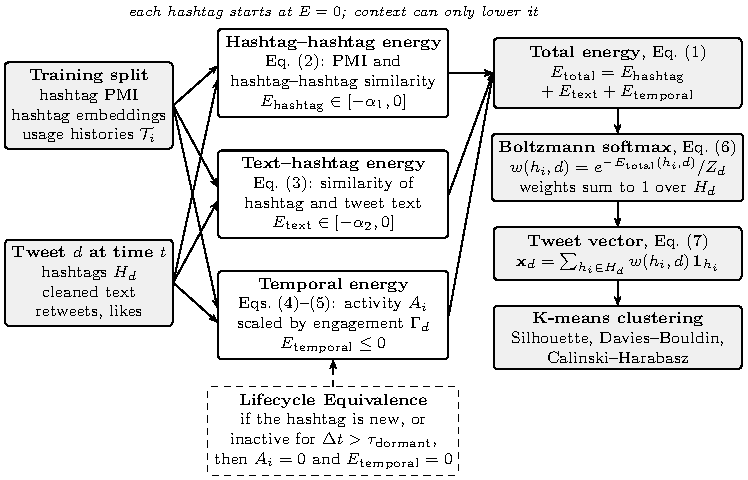
\includegraphics[width=\textwidth]{fig_framework.pdf}
\caption{Overview of the Zero-Energy Baseline framework. Every vocabulary hashtag $h_i$ of a tweet $d$ starts from zero energy, and three components can only lower it: co-occurrence (PMI) and semantic similarity with the other hashtags of the tweet (Eq.~\ref{eq:hashtag}), similarity with the tweet text (Eq.~\ref{eq:text}), and recent activity scaled by the engagement of the tweet (Eqs.~\ref{eq:activity}--\ref{eq:temporal}). The Lifecycle Equivalence rule (dashed box) sets the temporal energy of new and dormant hashtags to zero. A Boltzmann softmax over the hashtags of the tweet converts the total energies (Eq.~\ref{eq:total}) into weights that sum to one (Eq.~\ref{eq:weight}), and these weights form the sparse tweet vector clustered with K-means (Eq.~\ref{eq:representation}).}
\label{fig:framework}
\end{figure}

\subsection{The Zero-Energy Principle}\label{subsec8}

The foundational assumption of our framework is that hashtags possess \emph{no intrinsic importance}. This contrasts with frequency-based methods (TF-IDF, word counts), which implicitly assume that term importance is an inherent property determined by statistical regularities. Under the zero-energy principle, a hashtag without any contextual relationships has zero energy and therefore receives no preferential weight within its tweet.

Mathematically, every hashtag $h_i$ begins at a reference energy $E_{\text{rest}} = 0$. Deviations from this baseline arise only from interactions with other hashtags in the same tweet, with the surrounding text, and with temporal context. All energy components are non-positive, so more negative energy indicates stronger contextual support.

\subsection{Energy Decomposition}\label{subsec9}

We decompose the total contextual energy of hashtag $h_i$ in tweet $d$ posted at time $t$ into three components:
\begin{equation}
E_{\text{total}}(h_i, d) = E_{\text{hashtag}}(h_i, d) + E_{\text{text}}(h_i, d) + E_{\text{temporal}}(h_i, d, t)
\label{eq:total}
\end{equation}
Each component is weighted by a coefficient $\alpha_k \ge 0$ with $\alpha_1 + \alpha_2 + \alpha_3 = 1$. Only hashtags in the vocabulary (Section~\ref{subsec14}) are weighted.

\subsubsection{Hashtag-Hashtag Interaction Energy}\label{subsubsec1}

Hashtag co-occurrence patterns reveal topical structure: hashtags that frequently appear together likely belong to related topics. We model this through statistical association (Pointwise Mutual Information) and semantic similarity (embedding cosine similarity).

For hashtag $h_i$ in tweet $d$ with vocabulary hashtag set $H_d$, $|H_d| \ge 2$, the interaction energy is
\begin{equation}
E_{\text{hashtag}}(h_i, d) = -\alpha_1 \cdot \frac{1}{|H_d| - 1} \sum_{h_j \in H_d, j \neq i} \left[ \beta_1\, \widetilde{\text{PMI}}(h_i, h_j) + \beta_2\, \frac{1 + \cos(\mathbf{e}_{h_i}, \mathbf{e}_{h_j})}{2} \right]
\label{eq:hashtag}
\end{equation}
and $E_{\text{hashtag}}(h_i,d)=0$ when $|H_d| = 1$. Here $\text{PMI}(h_i, h_j) = \log \frac{P(h_i, h_j)}{P(h_i)P(h_j)}$ is estimated from co-occurrences in the training split, and $\widetilde{\text{PMI}}$ is its min--max normalisation to $[0,1]$ over all co-occurring training pairs; pairs that never co-occur in training receive $\widetilde{\text{PMI}} = 0$. Joint probabilities are estimated per tweet and marginal probabilities per hashtag occurrence; because $\widetilde{\text{PMI}}$ is min--max normalised, only the ordering of pairs matters. $\mathbf{e}_{h}$ is the embedding of hashtag $h$ produced by the sentence-transformer all-MiniLM-L6-v2~\cite{reimers2019}, with underscores replaced by spaces, and $\beta_1 = \beta_2 = 1/2$. Both bracketed terms lie in $[0,1]$, so $E_{\text{hashtag}} \in [-\alpha_1, 0]$.

PMI captures statistical co-occurrence, while semantic similarity captures relatedness even for hashtags that rarely co-occur in the training data.

\subsubsection{Text-Hashtag Coupling Energy}\label{subsubsec2}

If a hashtag aligns well with the tweet content, it is more likely to represent the tweet's topic. We model this through the similarity between the hashtag embedding and the tweet embedding:
\begin{equation}
E_{\text{text}}(h_i, d) = -\alpha_2 \cdot \frac{1 + \cos(\mathbf{e}_{h_i}, \mathbf{e}_{d})}{2}
\label{eq:text}
\end{equation}
where $\mathbf{e}_d$ is the all-MiniLM-L6-v2 sentence embedding of the cleaned tweet text (with hashtags, URLs and mentions removed). Hence $E_{\text{text}} \in [-\alpha_2, 0]$.

\subsubsection{Temporal Activity Energy}\label{subsubsec3}

Social media topics exhibit lifecycles of emergence, peak activity, decline and sometimes resurgence. We model a hashtag's current activity from its usage history $\mathcal{T}_i$, the set of timestamps of its occurrences in the training split. Let $t_{\text{last}}$ be the most recent element of $\mathcal{T}_i$ before $t$, and $\Delta t = t - t_{\text{last}}$. The activity of $h_i$ at time $t$ is
\begin{equation}
A_i(t) =
\begin{cases}
0 & \text{if } h_i \text{ has no earlier occurrence, or } \Delta t > \tau_{\text{dormant}} \\[2pt]
\rho_i(t)\, e^{-\Delta t / \tau_{\text{decay}}} & \text{otherwise}
\end{cases}
\label{eq:activity}
\end{equation}
where $\rho_i(t) = f_i(t-\Delta T, t) / f_i^{\max}$ is the number of occurrences of $h_i$ in the preceding window of length $\Delta T = 7$ days, divided by the maximum number of occurrences of $h_i$ in any 90-day window of the training split (a window longer than $\Delta T$), so that $\rho_i \in [0,1]$. The temporal energy scales this activity by the engagement of the tweet:
\begin{equation}
E_{\text{temporal}}(h_i, d, t) = -\alpha_3 \cdot A_i(t) \cdot \Gamma_d, \qquad \Gamma_d = \ln(1 + r_d + l_d)
\label{eq:temporal}
\end{equation}
where $r_d$ and $l_d$ are the retweet and like counts of tweet $d$. The engagement factor $\Gamma_d$ is non-negative but not bounded above, so $E_{\text{temporal}} \le 0$ without a fixed lower bound. In the Election 2020 test split, $\Gamma_d = 0$ for 49.1\% of tweets (which therefore receive no temporal energy), its mean is 0.81 and its maximum is 11.04. We use $\tau_{\text{dormant}} = 30$ days and $\tau_{\text{decay}} = 7$ days by default; their influence is examined in Section~\ref{subsec_sens}.

Two properties of Eq.~(\ref{eq:activity}) matter for interpretation. First, because $\rho_i(t)$ counts only uses in the last $\Delta T = 7$ days, a hashtag unseen for more than 7 days already has $A_i = 0$, so a dormancy threshold $\tau_{\text{dormant}} > \Delta T$ has no additional effect. Second, the usage history is built from the training split, so for test tweets $\Delta t$ is measured from a hashtag's last occurrence in the training period.

\subsection{Lifecycle Equivalence}\label{subsec10}

The \emph{Lifecycle Equivalence} rule states that a dormant hashtag (inactive for longer than $\tau_{\text{dormant}}$) is treated identically to a newly emerged hashtag: by Eq.~(\ref{eq:activity}) both have $A_i = 0$ and therefore zero temporal energy. Their weights then depend only on co-occurrence and text alignment. Because temporal energy is also zero whenever $\Gamma_d = 0$, which holds for about half of the Election 2020 test tweets, the rule mainly affects tweets with non-zero engagement.

The rule is designed for three situations. A new hashtag has no usage history; it starts with zero temporal energy, exactly as a dormant hashtag does, and can still receive weight through co-occurrence and text alignment, which addresses the cold-start problem. Hashtags that were once popular but have since become inactive do not retain temporal energy from past activity, which limits the effect of vocabulary drift. Finally, a hashtag that resurfaces after a period of dormancy rebuilds its temporal energy only from its renewed activity rather than from its historical popularity.

The reset is a hard threshold: temporal energy drops to zero once $\Delta t$ exceeds $\tau_{\text{dormant}}$. Whether the reset is exercised depends on the dataset's time span; we report this in Section~\ref{subsec_sens}.

\subsection{Weight Calculation and Normalization}\label{subsec11}

Given the total energy $E_{\text{total}}(h_i, d)$ for hashtag $h_i$ in tweet $d$, we convert energy to weight through a Boltzmann (softmax) distribution:
\begin{equation}
w(h_i, d) = \frac{\exp(-E_{\text{total}}(h_i, d))}{Z_d}, \qquad Z_d = \sum_{h_j \in H_d} \exp(-E_{\text{total}}(h_j, d))
\label{eq:weight}
\end{equation}
where $Z_d$ is the partition function normalizing weights across the vocabulary hashtags of tweet $d$. More negative energy yields higher weight, weights satisfy $w \in (0, 1]$ (with $w = 1$ when $|H_d| = 1$) and $\sum_{h_i \in H_d} w(h_i, d) = 1$, and they can be read as a probability distribution over the hashtags of each tweet.

The weighted hashtag representation of tweet $d$ is the sparse vector
\begin{equation}
\mathbf{x}_d = \sum_{h_i \in H_d} w(h_i, d) \cdot \mathbf{1}_{h_i}
\label{eq:representation}
\end{equation}
where $\mathbf{1}_{h_i}$ is the one-hot indicator of hashtag $h_i$ in the vocabulary. A tweet with no vocabulary hashtag is represented by the zero vector.

\subsection{Component Weighting and Parameter Selection}\label{subsec12}

In the absence of prior knowledge about which contextual relationship matters most, we assign equal weight to the three components, $\alpha_1 = \alpha_2 = \alpha_3 = 0.33$ (approximately $1/3$). For the temporal parameters we use $\tau_{\text{dormant}} = 30$ days and $\tau_{\text{decay}} = 7$ days, reflecting typical monthly and weekly timescales of social media discussion. Section~\ref{subsec_sens} reports a sensitivity analysis over 16 settings of $(\alpha_1, \alpha_2, \alpha_3)$ and 20 settings of $(\tau_{\text{dormant}}, \tau_{\text{decay}})$.

%%=============================================================%%
%% EXPERIMENTAL SETUP
%%=============================================================%%

\section{Experimental Setup}\label{sec4}

This section describes datasets, preprocessing, baseline methods, evaluation metrics, and statistical testing procedures.

\subsection{Datasets}\label{subsec13}

We evaluate on two Twitter datasets from different domains, scales and periods. Table~\ref{tab:splits} gives the size and period of each split.

\subsubsection{COVID-19 Health Discourse}\label{subsubsec4}

The COVID-19 dataset consists of three public collections of COVID-19 tweets covering April--June 2020, August--September 2020 and April--June 2021, published on Kaggle as the Covid-19 Twitter Dataset~\cite{covid_kaggle}. After filtering, it contains 41,949 tweets posted between 19 April 2020 and 27 June 2021, of which 6,293 form the test split. The vocabulary comprises 897 hashtags that occur at least 10 times in the training split, and tweets carry 3.2 hashtags on average (counting repeated hashtags). The discussion centres on pandemic response, vaccination, lockdowns, public health measures, variants and mask mandates.

\subsubsection{US Election 2020 Political Discourse}\label{subsubsec5}

The Election 2020 dataset~\cite{election_kaggle} was collected through the \#DonaldTrump and \#JoeBiden hashtags and captures political discourse around the 2020 US Presidential election. After filtering, it contains 1,216,987 tweets posted between 15 October and 8 November 2020, of which 182,549 form the test split; the test period (7--8 November) falls after election day. The vocabulary comprises 16,841 hashtags with at least 10 training occurrences, and tweets carry 2.8 hashtags on average (counting repeated hashtags). The discussion centres on the presidential candidates, voting processes, debates, campaign issues and swing states.

The two test sets differ 29-fold in size (6,293 vs 182,549 tweets) and 19-fold in vocabulary (897 vs 16,841 hashtags).

\begin{table}[t]
\centering
\caption{Chronological train/validation/test splits (70/15/15). All reported results are computed on the test split.}
\label{tab:splits}
\begin{tabular}{lccc}
\toprule
 & Train & Validation & Test \\
\midrule
\multicolumn{4}{l}{\textit{COVID-19}} \\
Tweets & 29,364 & 6,292 & 6,293 \\
Period & 19 Apr 2020 -- 16 May 2021 & 16 May -- 3 Jun 2021 & 3 -- 27 Jun 2021 \\
\midrule
\multicolumn{4}{l}{\textit{US Election 2020}} \\
Tweets & 851,890 & 182,548 & 182,549 \\
Period & 15 Oct -- 5 Nov 2020 & 5 -- 7 Nov 2020 & 7 -- 8 Nov 2020 \\
\bottomrule
\end{tabular}
\end{table}

\subsection{Preprocessing}\label{subsec14}

We apply identical preprocessing to both datasets. URLs, user mentions, numbers and special characters are removed from the tweet text, which is then converted to lowercase. Hashtags are extracted and lowercased separately and removed from the text used for TF-IDF and text embeddings. We retain tweets that contain at least two hashtags, to ensure co-occurrence signal, and more than 10 characters of cleaned text. Tweets are then sorted by timestamp and split 70/15/15 into training, validation and test sets without shuffling, so that every test tweet is later than every training tweet (Table~\ref{tab:splits}).

A hashtag enters the vocabulary if it occurs at least 10 times in the training split; hashtags outside the vocabulary are ignored. Only 4 of the 182,549 Election 2020 test tweets have no vocabulary hashtag, whereas in the COVID-19 test split this applies to 1,361 of 6,293 tweets (21.6\%), which are represented by the zero vector. PMI, hashtag usage histories and the TF-IDF vocabulary are computed on the training split only. Hashtags and tweet texts are embedded with the sentence-transformer all-MiniLM-L6-v2 (384 dimensions); because this model uses WordPiece subword tokenisation, every hashtag receives an embedding and no out-of-vocabulary fallback is needed.

The data were not de-duplicated; we discuss this in Section~\ref{subsec29}.

\subsection{Baseline Methods}\label{subsec15}

We compare against three baseline feature representations.

\subsubsection{TF-IDF Text-Only}\label{subsubsec6}

A bag-of-words representation of the cleaned tweet text (hashtags removed) using TF-IDF weighting with unigrams and bigrams, English stop-word removal, terms occurring in at least 5 and at most 80\% of training tweets, and the 5,000 most frequent remaining terms, fitted on the training split.

\subsubsection{Combined Hashtag-Text Features}\label{subsubsec7}

The L2-normalised contextual hashtag vector and the L2-normalised TF-IDF vector are each scaled by 0.5 and concatenated. This tests whether adding text features improves clustering.

\subsubsection{BERT Embeddings}\label{subsubsec8}

Contextual embeddings from bert-base-uncased~\cite{devlin2018}: the [CLS] token embedding (768 dimensions) of the final layer, without fine-tuning, computed once for the cleaned tweet text (maximum 128 tokens) and reused across all runs.

All representations are clustered with the same algorithm and evaluated with the same metrics. The BERT comparison (Table~\ref{tab:bert_comparison}) is performed at $K=20$ with five seeds.

\subsection{Clustering Algorithm}\label{subsec16}

We use K-means clustering (k-means++ initialization, 300 maximum iterations, 10 random restarts) for all experiments.

\subsection{Evaluation Metrics}\label{subsec17}

We employ three internal clustering metrics widely used in unsupervised learning~\cite{arbelaitz2013}.

The Silhouette score~\cite{rousseeuw1987} compares, for each point $i$, the average within-cluster distance $a_i$ with the average distance $b_i$ to the nearest other cluster:
\begin{equation}
s_i = \frac{b_i - a_i}{\max(a_i, b_i)}, \quad S = \frac{1}{N}\sum_i s_i
\end{equation}
It ranges from $-1$ to $1$, with higher values indicating better clustering. We use Euclidean distance and, for datasets larger than 10,000 tweets, a random sample of 10,000 points. Single-run values vary across seeds by about $\pm 0.007$, reflecting both the K-means initialisation and the random Silhouette sample; we therefore base conclusions on multi-seed results where they are available.

The Davies--Bouldin index~\cite{davies1979} averages, over all clusters, the similarity of each cluster to its most similar cluster, so lower values are better:
\begin{equation}
\text{DB} = \frac{1}{K}\sum_{i=1}^K \max_{j \neq i} \frac{\sigma_i + \sigma_j}{d_{ij}}
\end{equation}
where $\sigma_i$ is the average within-cluster distance for cluster $i$ and $d_{ij}$ is the distance between centroids $i$ and $j$.

The Calinski--Harabasz index~\cite{calinski1974} is the ratio of between-cluster to within-cluster dispersion, so higher values are better:
\begin{equation}
\text{CH} = \frac{N - K}{K - 1} \cdot \frac{\text{tr}(B)}{\text{tr}(W)}
\end{equation}

All three indices are computed in the feature space of each representation. They are therefore suited to comparing values of $K$ or parameter settings within one representation. Comparisons across representations (hashtag, TF-IDF, BERT) should be read with care, because each space has its own geometry; in particular, sparse representations with few non-zero entries can obtain high Silhouette values. We discuss this limitation in Section~\ref{subsec29}.

\subsection{Statistical Testing}\label{subsec18}

For the BERT comparison and the sensitivity analyses we perform five independent clustering runs with seeds 42--46 and report the mean and standard deviation across runs; the K-sensitivity and feature comparisons (Tables~\ref{tab:k_sensitivity} and~\ref{tab:feature_comparison}) are single runs with seed 42, and the ablation uses three seeds (Section~\ref{subsec22}). Normality of the per-run scores is checked with the Shapiro--Wilk test~\cite{shapiro1965}. Differences between methods are tested primarily with Welch's t-test~\cite{welch1947}, with the paired t-test (pairing runs by seed) as a secondary check, and with the Mann--Whitney U test~\cite{mann1947} as a non-parametric alternative; with five runs per group, the smallest attainable two-sided p-value of the latter is 0.008. We do not rely on the Wilcoxon signed-rank test, because with five paired runs its smallest attainable two-sided p-value is $2/32 = 0.0625$, so it cannot reach significance at the 0.05 level.

Effect sizes are reported as Cohen's $d = (\mu_1 - \mu_2)/\sigma_{\text{pooled}}$, using population standard deviations. Because the runs differ only in the K-means seed on a fixed dataset, the variance between runs is small and $d$ values are large; they measure stability across initialisations rather than sampling variability. In the sensitivity analyses, each setting is compared with the default using Welch's t-test with Holm correction~\cite{holm1979}, and all settings are compared jointly with a one-way ANOVA.

%%=============================================================%%
%% RESULTS
%%=============================================================%%

\section{Results}\label{sec5}

This section presents the K-sensitivity analysis (Section~\ref{subsec19}), feature type comparison (Section~\ref{subsec20}), BERT baseline comparison (Section~\ref{subsec21}), ablation study (Section~\ref{subsec22}), parameter sensitivity (Section~\ref{subsec_sens}) and a cross-domain summary (Section~\ref{subsec23}). Tables~\ref{tab:k_sensitivity} and~\ref{tab:feature_comparison} report single runs (seed 42); Tables~\ref{tab:bert_comparison}--\ref{tab:tau} report means over several seeds.

\subsection{K-Sensitivity Analysis}\label{subsec19}

We evaluate clustering quality for $K \in \{2, 5, 10, 15, 20\}$. Results for Hashtag-Only features appear in Table~\ref{tab:k_sensitivity}.

\begin{table}[t]
\centering
\caption{K-sensitivity of Hashtag-Only features (K-means, seed 42). Best value per column in bold.}
\label{tab:k_sensitivity}
\begin{tabular}{ccccc}
\toprule
\multirow{2}{*}{K} & \multicolumn{2}{c}{COVID-19} & \multicolumn{2}{c}{Election 2020} \\
\cmidrule(lr){2-3} \cmidrule(lr){4-5}
 & Silh.$\uparrow$ & DB$\downarrow$ & Silh.$\uparrow$ & DB$\downarrow$ \\
\midrule
2  & 0.2244 & 1.3387 & 0.1414 & 2.2389 \\
5  & 0.2640 & 1.3995 & 0.0955 & 2.4288 \\
10 & 0.3026 & 1.2986 & 0.1165 & \textbf{2.2161} \\
15 & 0.3108 & \textbf{1.2914} & 0.1200 & 2.2227 \\
20 & \textbf{0.3263} & 1.3946 & \textbf{0.1473} & 2.2885 \\
\bottomrule
\end{tabular}
\end{table}

COVID-19 reaches its highest Silhouette at $K=20$, a 45.4\% gain over $K=2$. For Election 2020 the highest single-run value is also at $K=20$, but it exceeds $K=2$ by only 0.006, which is within the run-to-run variation of about 0.007, so this dataset does not discriminate between these two values. Because $K=20$ is the largest value tested, we describe it as the best value within the tested range rather than as a global optimum. The two metrics do not fully agree, however: the Davies--Bouldin index is lowest at $K=15$ for COVID-19 and at $K=10$ for Election 2020, and for COVID-19 the value at $K=20$ is the second-worst (second-highest) of the five. This reflects the different weight the two indices give to cohesion and separation. We use $K=20$ in the remaining experiments because it is preferred by Silhouette for COVID-19 and is not worse for Election 2020, while noting that values between 10 and 20 are equally defensible by DB. Calinski--Harabasz values at $K=20$ are reported with the sensitivity analysis (Table~\ref{tab:alpha}).

The two datasets also differ in how quality changes with $K$. COVID-19 shows a monotonic increase in Silhouette from $K=2$ to $K=20$, whereas Election 2020 dips at $K=5$ before recovering. Election 2020 also has lower absolute scores (0.1473 vs 0.3263 at $K=20$), which is consistent with more heterogeneous discourse, generic hashtags such as \#Vote and \#Election2020, and overlapping communities.

\subsection{Feature Type Comparison}\label{subsec20}

Table~\ref{tab:feature_comparison} compares contextual hashtag features with TF-IDF and combined features, each at the $K$ with the highest Silhouette.

\begin{table}[t]
\centering
\caption{Feature comparison at each method's best $K$ by Silhouette (K-means, seed 42). $\Delta S$ is the absolute Silhouette difference to Hashtag-Only.}
\label{tab:feature_comparison}
\begin{tabular}{lcccccc}
\toprule
\multirow{2}{*}{Method} & \multicolumn{3}{c}{COVID-19} & \multicolumn{3}{c}{Election 2020} \\
\cmidrule(lr){2-4} \cmidrule(lr){5-7}
 & K & Silh. & $\Delta S$ & K & Silh. & $\Delta S$ \\
\midrule
Hashtag-Only & 20 & \textbf{0.3263} & -- & 20 & \textbf{0.1473} & -- \\
Combined     & 5  & 0.0891 & $-0.237$ & 2  & 0.0704 & $-0.077$ \\
TF-IDF-Only  & 15 & 0.0687 & $-0.258$ & 20 & 0.0303 & $-0.117$ \\
\bottomrule
\end{tabular}
\end{table}

Hashtag-Only features obtain the highest Silhouette in both datasets. Their advantage over TF-IDF features is 0.258 for COVID-19 and 0.117 for Election 2020, and over combined features 0.237 and 0.077. Adding TF-IDF features to the hashtag features therefore lowers Silhouette, from 0.3263 to 0.0891 for COVID-19 and from 0.1473 to 0.0704 for Election 2020; possible explanations are discussed in Section~\ref{subsec24}. Combined features also reach their highest Silhouette at smaller values of $K$ ($K=5$ for COVID-19 and $K=2$ for Election 2020) than Hashtag-Only features.

\subsection{BERT Baseline Comparison}\label{subsec21}

Table~\ref{tab:bert_comparison} compares contextual hashtag features with BERT [CLS] embeddings at $K=20$ over five seeds.

\begin{table}[t]
\centering
\caption{BERT baseline comparison at $K=20$ (mean $\pm$ population s.d. over seeds 42--46). Time is K-means clustering time only; it excludes the computation of hashtag weights and BERT embeddings. Shapiro--Wilk tests were run on the Election 2020 scores.}
\label{tab:bert_comparison}
\begin{tabular}{lcccc}
\toprule
 & \multicolumn{2}{c}{COVID-19} & \multicolumn{2}{c}{Election 2020} \\
\cmidrule(lr){2-3} \cmidrule(lr){4-5}
Method & Silh. & Time (s) & Silh. & Time (s) \\
\midrule
Hashtag-Only (Ours) & 0.3222$\pm$0.011 & 0.20 & 0.1424$\pm$0.006 & 6.2 \\
BERT [CLS]          & 0.0385$\pm$0.001 & 4.15 & 0.0726$\pm$0.001 & 147.8 \\
\midrule
$\Delta S$          & \multicolumn{2}{c}{$+0.284$} & \multicolumn{2}{c}{$+0.070$} \\
Paired $t$-test     & \multicolumn{2}{c}{$t$=50.05, $p<10^{-6}$} & \multicolumn{2}{c}{$t$=25.40, $p=1.4\times10^{-5}$} \\
Welch $t$-test      & \multicolumn{2}{c}{$p<10^{-5}$} & \multicolumn{2}{c}{$p=1.9\times10^{-5}$} \\
Mann--Whitney U     & \multicolumn{2}{c}{$p=0.008$} & \multicolumn{2}{c}{$p=0.008$} \\
Shapiro--Wilk $p$ (Ours / BERT) & \multicolumn{2}{c}{--} & \multicolumn{2}{c}{0.69 / 0.90} \\
Cohen's $d$         & \multicolumn{2}{c}{35.6} & \multicolumn{2}{c}{15.7} \\
\bottomrule
\end{tabular}
\end{table}

Contextual hashtag features score above BERT [CLS] embeddings by 0.284 Silhouette on COVID-19 and 0.070 on Election 2020. For Election 2020, Shapiro--Wilk tests do not reject normality of the per-run scores, so the t-tests are appropriate, and the Mann--Whitney U test reaches its smallest attainable value and leads to the same conclusion. The large Cohen's $d$ values reflect the low seed-to-seed variance of K-means on a fixed dataset.

This comparison has a limited scope. We use [CLS] embeddings without fine-tuning, which are a weak basis for clustering; pooled sentence embeddings or tweet-specific models such as BERTweet would be stronger baselines. Moreover, Silhouette is computed in each representation's own space, so the size of the difference should not be read as a difference in topic quality. In terms of cost, K-means on the sparse hashtag vectors is about 21 times (COVID-19) and 24 times (Election 2020) faster than on the dense 768-dimensional BERT vectors. This comparison covers the clustering step only: computing the hashtag weights also requires sentence-transformer embeddings, just as BERT requires encoding every tweet.

\subsection{Ablation Study: Hashtag/TF-IDF Mixing}\label{subsec22}

We vary the mixing weight $\lambda \in \{0.0, 0.25, 0.5, 0.75, 1.0\}$ between L2-normalised hashtag and TF-IDF features, concatenating $\lambda \times$ (hashtag features) and $(1-\lambda) \times$ (TF-IDF features), and run three clustering trials (seeds 42--44) at $K=20$ for each setting. Results for both datasets appear in Table~\ref{tab:ablation}. Because the hashtag vectors are L2-normalised here, the pure-hashtag scores differ from the unnormalised values in Tables~\ref{tab:k_sensitivity}--\ref{tab:bert_comparison}.

\begin{table}[t]
\centering
\caption{Ablation over hashtag/TF-IDF mixing ($K=20$, L2-normalised features, mean $\pm$ s.d. over three seeds; population s.d. for Election 2020 and sample s.d. for COVID-19). Rank within each dataset in parentheses.}
\label{tab:ablation}
\begin{tabular}{lcc}
\toprule
Configuration & COVID-19 Silh. & Election 2020 Silh. \\
\midrule
100\% Hash + 0\% TF  & \textbf{0.3445}$\pm$0.0054 (1) & \textbf{0.1049}$\pm$0.013 (1) \\
75\% Hash + 25\% TF  & 0.1681$\pm$0.1190 (2) & 0.0828$\pm$0.002 (2) \\
50\% Hash + 50\% TF  & 0.0572$\pm$0.0068 (5) & 0.0243$\pm$0.002 (4) \\
25\% Hash + 75\% TF  & 0.0657$\pm$0.0041 (4) & 0.0234$\pm$0.001 (5) \\
0\% Hash + 100\% TF  & 0.0714$\pm$0.0023 (3) & 0.0296$\pm$0.001 (3) \\
\bottomrule
\end{tabular}
\end{table}

Pure hashtag features score highest in both datasets, exceeding pure TF-IDF by 0.273 Silhouette on COVID-19 and 0.075 on Election 2020. The 25/75 and 50/50 mixtures score below pure TF-IDF in both domains, and the 75/25 mixture on COVID-19 is unstable across seeds (s.d. 0.119), which indicates that the clustering of the mixed space depends strongly on initialisation.

These results show that adding TF-IDF features does not help under the internal metrics used here. Possible explanations based on how the two blocks fill the concatenated space are discussed in Section~\ref{subsec24}.

\subsection{Parameter Sensitivity}\label{subsec_sens}

We examine the sensitivity of the framework to the component weights $(\alpha_1, \alpha_2, \alpha_3)$ and the temporal parameters $(\tau_{\text{dormant}}, \tau_{\text{decay}})$ on the full Election 2020 test split. For each setting, hashtag weights are recomputed for all 182,549 test tweets and K-means ($K=20$) is run with seeds 42--46. The default setting reproduces the feature matrix used in Tables~\ref{tab:k_sensitivity}--\ref{tab:bert_comparison} exactly. Its mean Silhouette here ($0.143 \pm 0.007$, sample s.d.) differs slightly from the $0.142$ in Table~\ref{tab:bert_comparison} because the 10,000-point Silhouette sample is drawn with a fixed seed in these runs but was not in the original runs.

We first vary the component weights $(\alpha_1, \alpha_2, \alpha_3)$ over the simplex in steps of 0.25, keeping $\tau_{\text{dormant}} = 30$ and $\tau_{\text{decay}} = 7$ days fixed (Table~\ref{tab:alpha}). Mean Silhouette ranges from 0.131 to 0.148, against $0.143 \pm 0.007$ for the default. No setting differs significantly from the default (Welch's t-test with Holm correction: all adjusted $p = 1.00$; smallest unadjusted $p = 0.074$), and a one-way ANOVA across all 16 settings gives $p = 0.34$. Davies--Bouldin (2.20--2.42) and Calinski--Harabasz (8,445--9,211) vary similarly little. The lowest mean value comes from the temporal component alone, whereas every setting that includes the hashtag or text component scores at least 0.132.

\begin{table}[t]
\centering
\caption{Sensitivity to the component weights (Election 2020, $K=20$, mean $\pm$ sample s.d. over seeds 42--46; $\tau_{\text{dormant}}=30$, $\tau_{\text{decay}}=7$ days).}
\label{tab:alpha}
\begin{tabular}{cccccc}
\toprule
$\alpha_1$ & $\alpha_2$ & $\alpha_3$ & Silhouette & DB & CH \\
\midrule
0.33 & 0.33 & 0.33 & 0.1430$\pm$0.0070 & 2.266 & 8,910 \\
1.00 & 0.00 & 0.00 & 0.1408$\pm$0.0086 & 2.333 & 9,164 \\
0.75 & 0.25 & 0.00 & 0.1374$\pm$0.0104 & 2.321 & 9,206 \\
0.75 & 0.00 & 0.25 & 0.1478$\pm$0.0078 & 2.208 & 9,039 \\
0.50 & 0.50 & 0.00 & 0.1363$\pm$0.0148 & 2.417 & 9,211 \\
0.50 & 0.25 & 0.25 & 0.1422$\pm$0.0093 & 2.269 & 9,015 \\
0.50 & 0.00 & 0.50 & 0.1379$\pm$0.0039 & 2.239 & 8,829 \\
0.25 & 0.75 & 0.00 & 0.1378$\pm$0.0048 & 2.350 & 9,091 \\
0.25 & 0.50 & 0.25 & 0.1366$\pm$0.0084 & 2.282 & 8,946 \\
0.25 & 0.25 & 0.50 & 0.1410$\pm$0.0103 & 2.214 & 8,828 \\
0.25 & 0.00 & 0.75 & 0.1402$\pm$0.0051 & 2.265 & 8,666 \\
0.00 & 1.00 & 0.00 & 0.1370$\pm$0.0082 & 2.310 & 9,127 \\
0.00 & 0.75 & 0.25 & 0.1423$\pm$0.0069 & 2.269 & 9,055 \\
0.00 & 0.50 & 0.50 & 0.1325$\pm$0.0105 & 2.319 & 8,727 \\
0.00 & 0.25 & 0.75 & 0.1384$\pm$0.0047 & 2.280 & 8,616 \\
0.00 & 0.00 & 1.00 & 0.1305$\pm$0.0113 & 2.201 & 8,445 \\
\bottomrule
\end{tabular}
\end{table}

We then vary $\tau_{\text{dormant}} \in \{1, 3, 7, 14, 30\}$ and $\tau_{\text{decay}} \in \{1, 3, 7, 14\}$ days with $\alpha_1 = \alpha_2 = \alpha_3 = 0.33$ (Table~\ref{tab:tau}). Mean Silhouette ranges from 0.135 to 0.144, against 0.143 for the default (30, 7), and no combination differs significantly from the default (all Holm-adjusted $p = 1.00$; smallest unadjusted $p = 0.061$; ANOVA $p = 0.69$).

\begin{table}[t]
\centering
\caption{Sensitivity to the temporal parameters (Election 2020, $K=20$, mean Silhouette over seeds 42--46; sample standard deviations 0.004--0.008).}
\label{tab:tau}
\begin{tabular}{lcccc}
\toprule
$\tau_{\text{dormant}}$ $\backslash$ $\tau_{\text{decay}}$ & 1 day & 3 days & 7 days & 14 days \\
\midrule
1 day   & 0.1396 & 0.1396 & 0.1396 & 0.1396 \\
3 days  & 0.1400 & 0.1416 & 0.1348 & 0.1400 \\
7 days  & 0.1376 & 0.1436 & 0.1430 & 0.1386 \\
14 days & 0.1376 & 0.1436 & 0.1430 & 0.1386 \\
30 days & 0.1376 & 0.1436 & 0.1430 (default) & 0.1386 \\
\bottomrule
\end{tabular}
\end{table}

Two patterns in Table~\ref{tab:tau} follow from Eq.~(\ref{eq:activity}). First, the rows for $\tau_{\text{dormant}} = 7$, 14 and 30 days are identical: because $\rho_i(t)$ counts only uses in the last $\Delta T = 7$ days, a hashtag unseen for more than 7 days already has zero activity, so thresholds above $\Delta T$ have no additional effect. Second, with $\tau_{\text{dormant}} = 1$ day, $\tau_{\text{decay}}$ has no effect: usage histories come from the training split and the test period begins about 1.8 days after training ends, so every test hashtag is reset to zero temporal energy, as the Lifecycle Equivalence rule prescribes. Switching off the temporal component in this way changes Silhouette by only 0.003. The Election 2020 corpus spans 25 days, so the default dormancy threshold of 30 days is not exercised on this dataset.

A further reason for the stability in Tables~\ref{tab:alpha} and~\ref{tab:tau} is that, in practice, the energies of the hashtags within a tweet differ little relative to the softmax scale (the hashtag and text energies are bounded by $\alpha_1$ and $\alpha_2$, and the temporal energy is zero for about half of the tweets), so the weights within a tweet stay close to uniform: on the Election 2020 test split, the largest deviation of a tweet's weights from $1/|H_d|$ averages 0.014 (95th percentile 0.047). Consistent with this, replacing the energy weights by uniform weights $1/|H_d|$ gives Silhouette $0.149 \pm 0.004$ against $0.143 \pm 0.007$ for the energy weights (Welch $p = 0.14$), while binary hashtag indicators give $0.105 \pm 0.005$ (Election 2020, $K=20$, seeds 42--46, sample s.d.). To compare the contextual weights directly with frequency-based weighting, we also weight each hashtag by its inverse document frequency in the training split, $\mathrm{idf}(h) = \ln\bigl(N/(1+\mathrm{df}(h))\bigr) + 1$, on the same vocabulary and with the same protocol. Normalised to sum to one within each tweet, as the energy weights are, IDF weights give $0.138 \pm 0.025$, which does not differ from the energy weights (Welch $p = 0.67$) but varies considerably across seeds; with the L2 normalisation usual for TF-IDF they give $0.124 \pm 0.005$ ($p = 0.001$). Under the same per-tweet normalisation, therefore, neither the contextual nor the frequency-based weights improve on uniform weighting, and the normalisation affects Silhouette more than the choice of weights. Figure~\ref{fig:weighting} shows the per-seed scores: the energy, uniform and per-tweet normalised IDF weights overlap, and the IDF weights vary most across seeds.

\begin{figure}[t]
\centering
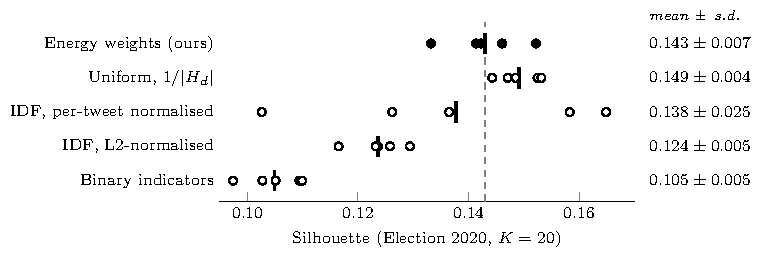
\includegraphics{fig_weighting.pdf}
\caption{Silhouette of five hashtag weighting schemes on Election 2020 ($K=20$, K-means, seeds 42--46), all using the same vocabulary, test tweets and clustering protocol. Each dot is one seed and the vertical bar marks the mean; the dashed line marks the mean of the energy weights. Values on the right are the mean and sample standard deviation over seeds. The energy, uniform and per-tweet normalised IDF weights overlap, whereas the L2-normalised IDF weights and binary indicators score lower.}
\label{fig:weighting}
\end{figure}

\subsection{Cross-Domain Summary}\label{subsec23}

Table~\ref{tab:cross_domain} summarises the results for both datasets.

\begin{table*}[t]
\centering
\caption{Cross-domain summary of the results}
\label{tab:cross_domain}
\footnotesize
\begin{tabular}{lccl}
\toprule
Result & COVID-19 & Election 2020 & Note \\
\midrule
Highest Silhouette & Hashtag-Only & Hashtag-Only & Same in both \\
Best $K$ by Silhouette (tested range) & 20 & 20 ($\approx K=2$) & DB prefers 15 and 10 \\
$\Delta S$ Hashtag vs Combined & $+0.237$ & $+0.077$ & Same direction \\
$\Delta S$ Hashtag vs TF-IDF & $+0.258$ & $+0.117$ & Same direction \\
$\Delta S$ Hashtag vs BERT [CLS] & $+0.284$ & $+0.070$ & $p<0.001$ in both \\
K-means speed-up vs BERT & $\approx$21$\times$ & $\approx$24$\times$ & Clustering step only \\
Ablation: best mixture & 100\% Hash & 100\% Hash & Same in both \\
Sensitivity to $\alpha$, $\tau$ & -- & Not significant & Election 2020 only \\
\midrule
Silhouette, Hashtag-Only (5 seeds) & 0.32 & 0.14 & Domain difficulty \\
Combined features, best $K$ & 5 & 2 & Differs \\
K pattern & Monotonic & Dip at $K=5$ & Differs \\
\bottomrule
\end{tabular}
\end{table*}

In both datasets, Hashtag-Only features score above Combined and TF-IDF features and above BERT [CLS] embeddings, and the ablation ranks pure hashtag features first. The relative ordering is therefore consistent across health and political discourse, although with two datasets this supports consistency rather than general claims about other domains. Absolute Silhouette values, by contrast, differ substantially (0.32 vs 0.14 for Hashtag-Only, five-seed means in Table~\ref{tab:bert_comparison}). Health discourse has a more homogeneous topical structure, whereas political discourse contains generic hashtags, polarised communities and noise; part of the COVID-19 value may also reflect the 21.6\% of test tweets represented by the zero vector (Section~\ref{subsec29}). Both datasets use identical hyperparameters ($\tau_{\text{dormant}}=30$ days, $\tau_{\text{decay}}=7$ days, $\alpha_1=\alpha_2=\alpha_3=0.33$) without domain-specific tuning, and the sensitivity analysis indicates that the Election 2020 results do not depend on these choices.

%%=============================================================%%
%% DISCUSSION
%%=============================================================%%

\section{Discussion}\label{sec6}

This section interprets the results, discusses practical considerations, and sets out the limitations.

\subsection{Why Hashtag-Only Scores Above Combined Features}\label{subsec24}

Adding TF-IDF features lowers Silhouette in both datasets, and several explanations are possible that our experiments do not distinguish. Under the zero-energy view, hashtag weights encode contextual importance while TF-IDF encodes frequency-based, intrinsic importance, so combining the two may produce a feature space in which neither notion is represented consistently. A second explanation concerns signal and noise: hashtags are curated metadata chosen by users to label topics, whereas tweet text contains typos, slang, emotional expressions and off-topic content, so adding noisier features to cleaner ones can dilute the signal.

A third explanation is geometric. The combined features have 5,897 dimensions for COVID-19 (897 hashtags and 5,000 TF-IDF terms) and 21,841 for Election 2020. Both blocks are L2-normalised and weighted equally, but the TF-IDF block spreads its mass over more, less informative dimensions, so distances in the concatenated space become less discriminative, which by itself can lower Silhouette. Testing these explanations, for example by re-weighting the blocks to equal variance or by evaluating with an external, representation-independent measure, is left for future work.

\subsection{Why BERT [CLS] Embeddings Score Lower}\label{subsec25}

Several factors may explain why BERT [CLS] embeddings score lower. BERT is pre-trained on Wikipedia and BookCorpus, whose formal, well-edited text differs from informal tweets with non-standard orthography and platform conventions. Because clustering is unsupervised, we use the [CLS] embeddings without task-specific adaptation, and such embeddings are known to represent sentence similarity poorly; pooled or sentence-level models would probably perform better. The hashtag representation, in contrast, is designed for topic clustering and relies on user-curated labels rather than on the full, noisy text. Finally, Silhouette is computed in a 768-dimensional dense space for BERT and in a sparse space with few non-zero entries for hashtags, so the difference in scores reflects the geometry of the two spaces as well as clustering quality.

\subsection{Choice of K}\label{subsec26}

Within the tested range, Silhouette is highest at $K=20$ for COVID-19 and does not separate $K=2$ from $K=20$ for Election 2020, while Davies--Bouldin favours $K=15$ (COVID-19) and $K=10$ (Election 2020). Values of $K$ between 10 and 20 therefore appear appropriate for these datasets, and larger values were not tested. COVID-19 discourse spans vaccines, treatments, prevention, social impacts and variants (e.g., Alpha and Delta, which circulated during the collection period); Election 2020 spans candidates, issues, voting processes and events. The gain from $K=2$ to $K=20$ is 45\% for COVID-19, whereas for Election 2020 it is within run-to-run variation. For human interpretation, fine-grained clusters can be grouped hierarchically into coarser categories.

\subsection{Consistency Across Domains}\label{subsec27}

The relative ordering of representations is the same for health and political discourse, despite a 29-fold difference in test-set size and a 19-fold difference in vocabulary. This suggests that the ordering is not specific to one domain or scale. With two English-language Twitter datasets, however, the results support consistency between these settings rather than generalisation to other platforms, languages or domains.

\subsection{Practical Considerations}\label{subsec28}

On the sparse hashtag vectors, K-means runs about 21--24 times faster than on dense BERT vectors. The full pipeline, however, also requires sentence-transformer embeddings for hashtags and tweets, PMI statistics and usage histories; these can be computed offline and updated incrementally, but we did not measure end-to-end or streaming performance. The resources involved are modest: the all-MiniLM-L6-v2 model (about 90\,MB), a sparse PMI matrix whose size depends on the vocabulary, and hashtag usage timestamps. The energy decomposition also attributes each hashtag weight to co-occurrence, text alignment and temporal activity; because the weights stay close to uniform on these datasets, however, this attribution explains little of the cluster assignments. Since the sensitivity analysis on Election 2020 shows no significant change across the tested component weights and temporal parameters, extensive hyperparameter search does not appear necessary, although this insensitivity is also consistent with the near-uniform weights and was tested on one dataset only.

\subsection{Limitations and Future Directions}\label{subsec29}

The evaluation has several limitations. All results rely on internal validity indices, and no human-annotated topic labels are available. These indices are computed in each representation's own space, and sparse representations with few non-zero entries can obtain high Silhouette values, so differences between representations should be interpreted with care. Future work should add external evaluation, such as topic coherence or human annotation, and downstream tasks such as retrieval or trend detection. The BERT [CLS] baseline without fine-tuning is also weak, and comparisons with sentence-level and tweet-specific models (Sentence-BERT, BERTweet) and with BERTopic would strengthen the evaluation.

A second group of limitations concerns the method itself. Because the energies of the hashtags within a tweet differ little in practice, the Boltzmann weights within a tweet remain close to uniform (Section~\ref{subsec_sens}). On Election 2020, uniform weights perform on par with the energy weights, and IDF weights normalised in the same way do not differ from them (Section~\ref{subsec_sens}), so the advantage over TF-IDF and BERT stems mainly from the hashtag representation and its per-tweet normalisation rather than from the contextual weighting. Making the weights more selective, for example through a temperature parameter in Eq.~(\ref{eq:weight}), is a direction for future work. The temporal component is also only partly exercised: the Election 2020 corpus spans 25 days, so the dormancy reset at $\tau_{\text{dormant}} = 30$ days never applies, thresholds above the 7-day activity window have no effect, and the engagement factor $\Gamma_d$ is zero for about half of the Election 2020 test tweets, which therefore receive no temporal energy.

A third group concerns the data. Only English Twitter data from two events is used, so further domains, platforms and languages are needed before broader claims can be made. Only tweets with at least two hashtags are included, and tweets without hashtags cannot be clustered by the method. In the COVID-19 test split, 21.6\% of tweets have no hashtag in the training vocabulary and are represented by the zero vector; because identical vectors cluster tightly, this can raise Silhouette, and the COVID-19 Hashtag-Only score should be read with that caveat. The data were also not de-duplicated, and the Election 2020 corpus contains repeated tweets, including tweets collected under both candidate hashtags. The same mechanism applies here: 23\% of the Election 2020 test tweets have a hashtag vector identical to that of an earlier test tweet, either because the tweet is repeated or because its hashtag set is. Removing these rows and the four empty rows lowers the Hashtag-Only Silhouette at $K=20$ from 0.143 to 0.091 (seeds 42--46), and uniform weights give 0.089 on the same reduced set. The absolute Silhouette values for Election 2020 are therefore inflated by repeated hashtag vectors; we did not re-run the baselines on the reduced set, so the effect on the comparison with the other representations is not known. Finally, the framework produces a flat clustering of a static test split; hierarchical clustering and streaming algorithms with incremental updates are natural extensions.

%%=============================================================%%
%% CONCLUSION
%%=============================================================%%

\section{Conclusion}\label{sec7}

This paper introduced a Zero-Energy Baseline framework for contextual hashtag weighting in social media clustering and evaluated it on COVID-19 health discourse (6,293 test tweets) and US Election 2020 political discourse (182,549 test tweets). In the framework, hashtags have no intrinsic importance; their weights are derived from co-occurrence, alignment with the tweet text and engagement-scaled temporal activity, with dormant and new hashtags treated identically under the Lifecycle Equivalence rule.

In both datasets, contextual hashtag features obtain higher Silhouette than TF-IDF features, concatenated hashtag--TF-IDF features and BERT [CLS] embeddings, and pure hashtag features rank first in an ablation over mixing weights. Within the tested range, Silhouette is highest at $K=20$ for COVID-19, while for Election 2020 it does not separate $K=2$ from $K=20$ and Davies--Bouldin favours $K$ between 10 and 15. On Election 2020, sensitivity analyses over 16 settings of the component weights and 20 settings of the temporal parameters show no significant change in clustering quality.

These results are consistent across two domains that differ substantially in scale and topic. They are based on internal validity indices, two English-language Twitter datasets and a K-means pipeline. On Election 2020, the contextual weights perform on par with uniform weights, so the gains are attributable mainly to the hashtag representation. Future work will add external evaluation, stronger embedding baselines, more selective weighting, further domains, and hierarchical and streaming variants.

%%=============================================================%%
%% BACKMATTER
%%=============================================================%%

\backmatter

\bmhead{Acknowledgments}

The authors thank Sharda University, Greater Noida, India; INTI International University, Malaysia; Sivas University of Science and Technology, Türkiye; and British University Vietnam for providing computing facilities.

\section*{Declarations}

\textbf{Funding:} No external funding was received for this research.

\textbf{Conflict of interest:} The authors declare that they have no conflict of interest.

\textbf{Ethics approval:} This research uses publicly available Twitter datasets and does not involve human subjects experimentation. No ethics approval was required.

\textbf{Data availability:} Both datasets are publicly available: the COVID-19 tweets from~\cite{covid_kaggle} and the Election 2020 tweets from~\cite{election_kaggle}. The code, fixed random seeds and result files needed to reproduce all tables are available at \url{https://github.com/batri80/Contextual-Hashtag-Weighting}, and the preprocessing script rebuilds the chronological splits from the two public collections. Tweet text is not redistributed, in line with the platform's terms of use, and tweet identifiers are not provided because the files we processed hold them only as rounded floating-point values (the Election 2020 collection itself stores them in this form).

\textbf{Author contributions:} KB conceived the framework and led the research. RT, CA, PS, MVP, SL, and SM contributed to experimental design, implementation, analysis, and manuscript preparation. All authors reviewed and approved the final manuscript.

%%=============================================================%%
%% BIBLIOGRAPHY
%%=============================================================%%

\bibliography{reference}

\end{document}
